% $Header: /data/cvsroot/Courses/OnlineLearning/talks/talk4/talk4.tex,v 1.4 2006/01/24 08:08:47 yfreund Exp $

%\documentclass{beamer}
\documentclass[handout]{beamer}
% This file is a solution template for:
% - Giving a talk on some subject.
% - The talk is between 15min and 45min long.
% - Style is ornate.

% Copyright 2004 by Till Tantau <tantau@users.sourceforge.net>.
%
% In principle, this file can be redistributed and/or modified under
% the terms of the GNU Public License, version 2.
%
% However, this file is supposed to be a template to be modified
% for your own needs. For this reason, if you use this file as a
% template and not specifically distribute it as part of a another
% package/program, I grant the extra permission to freely copy and
% modify this file as you see fit and even to delete this copyright
% notice. 


\mode<presentation>
{
  \usetheme{Montpellier}

  %\setbeamercovered{transparent}
  % or whatever (possibly just delete it)
}

\usepackage{xmpmulti} % package that defines \multiinclude

\usepackage[english]{babel}

\usepackage[latin1]{inputenc}

\usepackage{times}
\usepackage[T1]{fontenc}
% Or whatever. Note that the encoding and the font should match. If T1
% does not look nice, try deleting the line with the fontenc.

\title[Internal Regret and Calibration]% (optional, use only with long paper titles)
{Internal Regret \\ and \\ Calibration}

\author[Freund] % (optional, use only with lots of authors)
{Yoav Freund}
% - Give the names in the same order as the appear in the paper.
% - Use the \inst{?} command only if the authors have different
%   affiliation.

\institute[Universities of Somewhere and Elsewhere] % (optional, but mostly needed)

\subject{Machine Learning}
% This is only inserted into the PDF information catalog. Can be left
% out. 

% If you have a file called "university-logo-filename.xxx", where xxx
% is a graphic format that can be processed by latex or pdflatex,
% resp., then you can add a logo as follows:

% \pgfdeclareimage[height=0.5cm]{university-logo}{university-logo-filename}
% \logo{\pgfuseimage{university-logo}}



% Delete this, if you do not want the table of contents to pop up at
% the beginning of each subsection:
%% \AtBeginSubsection[]
%% {
%%   \begin{frame}<beamer>
%%     \frametitle{Outline}
%%     \tableofcontents[currentsection,currentsubsection]
%%   \end{frame}
%% }


% If you wish to uncover everything in a step-wise fashion, uncomment
% the following command: 

\beamerdefaultoverlayspecification{<+->}

%\newcommand{\R}[1]{{\color{red}{#1}}}
%\newcommand{\vp}{{\mathbf p}}
%\newcommand{\HedgeLoss}{L_{\mbox{\footnotesize Hedge}}}

\newcommand{\newmcommand}[2]{\newcommand{#1}{{\ifmmode {#2}\else\mbox{${#2}$}\fi}}}
\newcommand{\renewmcommand}[2]{\renewcommand{#1}{{\ifmmode {#2}\else\mbox{${#2}$}\fi}}}
\newcommand{\newmcommandi}[2]{\newcommand{#1}[1]{{\ifmmode {#2}\else\mbox{${#2}$}\fi}}}
\newcommand{\newmcommandii}[2]{\newcommand{#1}[2]{{\ifmmode {#2}\else\mbox{${#2}$}\fi}}}
\newcommand{\newmcommandiii}[2]{\newcommand{#1}[3]{{\ifmmode {#2}\else\mbox{${#2}$}\fi}}}

\newcommand{\algfnt}{\bf}

\newmcommand{\ouralg}{{\mbox{\algfnt Hedge}({\eta})}}

\newmcommand{\iter}{T}

\newfont{\cmmib}{cmmib10}
\newcommand{\boldell}{{\mbox{\cmmib \symbol{'140}}}}


\newmcommandi{\costvec}{{\boldell}_{#1}}
\newmcommandii{\cost}{{\ell}^{#1}_{#2}}

\newmcommandi{\rd}{\tilde{#1}}

\newmcommandi{\distvec}{{\bf p}^{#1}}
\newmcommandi{\rddistvec}{\rd{\bf p}^{#1}}
\newmcommandii{\dist}{{p}^{#1}_{#2}}
\newmcommandii{\rddist}{\rd{p}^{#1}_{#2}}

\newmcommandi{\bdistvec}{{\bf q}^{#1}}
\newmcommandii{\bdist}{{q}^{#1}_{#2}}

\newmcommandi{\wtvec}{{\bf w}^{#1}}
\newmcommandi{\rdwtvec}{\rd{\bf w}^{#1}}
\newmcommandii{\wt}{{w}^{#1}_{#2}}
\newmcommandii{\rdwt}{\rd{w}^{#1}_{#2}}


\newcommand{\Nweight}[2]{V_{#1}^{#2}}	%the normalized weight
\newcommand{\dweight}[2]{w^{#2}(#1)} % initial density measure
\newcommand{\TEloss}[1]{L_{#1}}	%total loss of expert i
\newcommand{\BEloss}{L_{\min}}	%total loss of the best expert
\newcommand{\TAloss}{L_A}	%total loss of algorithm
\newcommand{\weight}[2]{W_{#1}^{#2}} % weight assigned to expert
\newcommand{\btheta}{\hat{\theta}}

\newcommand{\R}[1]{{\color{red}{#1}}}
\newcommand{\B}[1]{{\color{blue}{#1}}}
\newcommand{\RM}[1]{{\color{red}{$#1$}}}


%BANDITS
\newcommand{\Aplay}{{\bf Hedge}}
\newcommand{\Aest}{{\bf Exp3}}
\newcommand{\Aesthp}{{\bf Exp3.P}}
\newcommand{\Aestg}{{\bf Exp3.P.1}}
\newcommand{\Aests}{{\bf Exp3.S}}
\newcommand{\Aessg}{{\bf Exp3.S.1}}
\newcommand{\Astrat}{{\bf Exp4}}
\newcommand{\Abound}{{\bf Exp3.1}}
\newcommand{\Gbest}{G_{\rm max}}

\newcommand{\defeq}{\stackrel{\rm def}{=}}
\newcommand{\compl}{\mbox{\sc h}}
\newcommand{\theset}[2]{\{ {#1} \,:\, {#2} \}}

\newmcommandii{\stratv}{\mbox{\boldmath $\xi$}^{#1}({#2})}

%Games paper
\newmcommand{\M}{\bf M}
\newmcommand{\dM}{\M'}
\newmcommand{\Row}{\bf R}
\newmcommand{\dRow}{\R'}
\newmcommand{\C}{\bf C}
\newmcommand{\dC}{\C'}
\newmcommand{\D}{D}
\renewmcommand{\P}{\bf P}
\newmcommand{\Q}{\bf Q}
\newmcommand{\Dt}{\D_t}
\newmcommand{\Pt}{\P_t}
\newmcommand{\Qt}{\Q_t}
\newmcommand{\Pstar}{\P^*}	% the min/max optimal mixed strategy
\newmcommand{\Pref}{\tilde{\P}}	% a reference mixed strategy (not
				% necessarily min/max)
\newmcommand{\Qstar}{\Q^*}
\newmcommand{\Pa}{\overline{\P}}
\newmcommand{\Qa}{\overline{\Q}}
\newmcommand{\Qh}{\hat{\Q}}
\newmcommandi{\trans}{{#1}^{\rm T}}
\newmcommand{\mhx}{\M(h,x)}
\newmcommand{\mxh}{\dM(x,h)}
\newmcommand{\mpq}{\M(\P,\Q)}
\newmcommand{\mpsq}{\M(\Pstar,\Q)}
\newmcommand{\mpsqt}{\M(\Pstar,\Qt)}
\newmcommand{\mptqt}{\M(\Pt,\Qt)}
\newmcommand{\mptt}{\M(\Pt,t)}
\newmcommand{\mptq}{\M(\Pt,\Q)}
\newmcommand{\mpqt}{\M(\P,\Qt)}
\newcommand{\minp}{\min_{\P}}
\newcommand{\maxq}{\max_{\Q}}
\newcommand{\RE}[2]{{\rm RE}\left( {#1} \; \parallel \; {#2} \right) }

\newmcommand{\sumt}{\sum_{t=1}^T}
\newmcommand{\sumin}{\sum_{i=1}^n}
\newmcommand{\delt}{\Delta_{T,n}}
\newcommand{\nextline}{\vspace{0.2cm}\\}   % a little space for equation arrays

\newcommand{\lwalg}{\mbox{\rm MW}}
\newcommand{\lwalgvar}{\mbox{\rm vMW}}

%%
\newcommand{\E}{\mbox{\rm\bf E}}
\newcommand{\p}[2]{p_{#1}(#2)}
\newcommand{\q}[2]{q_{#1}(#2)}
\newcommand{\x}[2]{x_{#1}({#2})}
\newmcommand{\bx}{\mbox{\boldmath$x$}}
\newmcommandi{\xv}{\bx({#1})}
\newmcommand{\xvt}{\xv{t}}
%\newcommand{\w}[2]{w_{#1}({#2})} replaced by \wt, but remember to switch order of parameters i and t
\renewcommand{\i}[1]{i_{#1}}
\newcommand{\hx}[2]{\hat{x}_{#1}(#2)}
\newcommand{\hxit}{\hx{\i{t}}{t}}
\newcommand{\pit}{\p{\i{t}}{t}}
\newcommand{\xit}{\x{\i{t}}{t}}
\newcommand{\expb}[1]{\exp\left(#1\right)}

\newcommand{\vp}{{\mathbf p}}
\newcommand{\vu}{{\mathbf u}}
\newcommand{\vv}{{\mathbf v}}
\newcommand{\vx}{{\mathbf x}}
\newcommand{\vy}{{\mathbf y}}
\newcommand{\vw}{{\mathbf w}}
\newcommand{\vz}{{\mathbf z}}
\newcommand{\vq}{{\mathbf q}}
\newcommand{\vg}{{\mathbf g}}

\newcommand{\vecq}{{\bf q}}
\newcommand{\vecp}{{\bf p}}


\newcommand{\HedgeLoss}{L_{\mbox{\footnotesize Hedge}}}

\newcommand{\W}{\vec{W}}
\newcommand{\V}{\vec{V}}
\newcommand{\X}{\vec{X}}
\newcommand{\vb}{\vec{b}}
%\newcommand{\loss}{\vec{\ell}}
\newcommand{\loss}{L}
\newcommand{\elloss}[2]{\ell_{#2}\left( #1 \right)} %loss of expert i at time t
\newcommand{\lossvec}[1]{{\mathbf \ell}_{#1}}       %loss of expert at time t
\newcommand{\w}[1]{\makebox[12pt]{{#1}}}
\newcommand{\Rps}{\mbox{\tt R}}
\newcommand{\rPs}{\mbox{\tt P}}
\newcommand{\rpS}{\mbox{\tt S}}
\newcommand{\rpstie}{\w{$\frac{1}{2}$}}
\newcommand{\rpswin}{\w{$0$}}
\newcommand{\rpsloss}{\w{$1$}}

\newmcommand{\decspace}{\Delta}
\newmcommand{\decsym}{\delta}
\newmcommandi{\dec}{\decsym^{#1}}
\newmcommand{\decdistsym}{\cal D}
\newmcommandi{\decdist}{{\decdistsym}^{#1}}

\newmcommand{\simpdistspace}{{\bf \cal S}}
\newmcommand{\domset}{{\rm dom}(\decdistsym)}

\newmcommand{\expdistsym}{{\cal E}}
\newmcommandii{\expdist}{{\expdistsym}^{#1}_{#2}}
\newmcommand{\expdecsym}{{\varepsilon}}
\newmcommandii{\expdec}{\expdecsym^{#1}_{#2}}

\newmcommand{\outspace}{\Omega}
\newmcommand{\outsym}{\omega}
\newmcommandi{\out}{\outsym^{#1}}

%\newmcommandii{\Dkl}{D_{\mbox{kl}}\paren{#1||#2}}
\newmcommandii{\Dkl}{{\rm {KL}}\paren{{#1}\;||\;{#2}}}

\newmcommandi{\sumwts}{\sum_{i=1}^N \wt{#1}{i}}

\newmcommand{\lossalg}{L_A}
\newmcommand{\lossouralg}{{L_{\mbox{\scriptsize\algfnt Hedge}(\eta)}}}
\newmcommand{\lossS}{{L_{\mbox{\scriptsize\algfnt S}}}}
\newmcommandi{\lossi}{L_{#1}}
\newmcommandii{\lossit}{L_{#1}^{#2}}

\newmcommandi{\upbnd}{\tilde{#1}}

\newcommand{\angles}[1]{{\left\langle {#1} \right\rangle}}
\newcommand{\paren}[1]{{\left( {#1} \right)}}
\newcommand{\brac}[1]{{\left[ {#1} \right]}}
\newcommand{\braces}[1]{{\left\{ {#1} \right\}}}

\newcommand{\abs}[1]{{\left| {#1} \right|}}
\newcommand{\ceiling}[1]{{\left\lceil {#1} \right\rceil}}

\newfont{\msym}{msbm10}
\newcommand{\real}{\mbox{\msym R}}

\newmcommand{\updatefcn}{U_\eta}

%% \newtheorem{theorem}{Theorem}	
%% \newtheorem{lemma}[theorem]{Lemma}
%% \newtheorem{corollary}[theorem]{Corollary}
%% \newtheorem{definition}{Definition}

%\newcommand{\proof}{\noindent{\bf Proof:} }
%\newcommand{\example}[1]{{\em Example #1.} }
%\newcommand{\qed}{\rule{0.7em}{0.7em}}

\newcommand{\WeakAlg}{\mbox{\algfnt WeakLearn}}
\newcommand{\Boost}{\mbox{\algfnt AdaBoost}}
\newcommand{\EX}{\mbox{\bf EX}}
\newmcommand{\hf}{h_{{f}}}
\newmcommand{\rdhf}{\rd{h}_{{f}}}
\newmcommand{\hfT}{h^T_{{f}}}
\newmcommand{\ranh}{{b}}

\newmcommand{\conclass}{{\cal C}}

\newmcommand{\badvec}{{\bf b}}
\newmcommandi{\bad}{{b}_{#1}}

%%%%%%%% New commands defined for the game-playing paper

\newmcommand{\hedge}{\algfnt Hedge}
\newmcommand{\play}{\algfnt Play}
\newmcommandi{\Glossvec}{{\bg y}^{#1}}
\newmcommandii{\Gloss}{{y}^{#1}_{#2}}
%\newmcommandi{\action}{{I}_{#1}}
\newmcommandi{\Gdistvec}{{\bf \tilde{p}}^{#1}}
\newmcommandii{\Gdist}{{\teilde{p}}^{#1}_{#2}}

%%%%%%%%%%%%%%%%%%%%%%%%%%%%%%%%%%%%%%%%%%%%%%%%%%%%%
\newmcommand{\Idistvec}{{D}}
\newmcommandi{\Idist}{\Idistvec({#1})}
\newmcommand{\Idistt}{\Idistvec_t}

\newmcommand{\Xdist}{{\cal P}}
\newmcommand{\emp}{\hat{\epsilon}}

\newmcommand{\classpc}{Y}
\newmcommand{\numclass}{k}
\newmcommandii{\prob}{\mbox{\rm Pr}_{#1}\left[{#2}\right]}
\newmcommandii{\exval}{\mbox{\rm E}_{#1}\left[{#2}\right]}

%\usepackage{amsmath}
\DeclareMathOperator*{\argmax}{argmax} % thin space, limits underneath in displays
\DeclareMathOperator*{\argmin}{argmin} 

\newcommand{\RR}{{\mathbf R}}
\newcommand{\rr}{{\mathbf r}}
\newcommand{\Btheta}{\bm{\theta}}
\newcommand{\regret}{\mbox{Regret}}

%%% Conditional probabilities
\newmcommandii{\condp}{p\left( #1 \left| #2 \right. \right)}

\newmcommand{\lab}{y}
\newmcommand{\ploss}{\mbox{ploss}}
\newmcommandii{\avploss}{\ploss_{#1}({#2})}
\newcommand{\sfrac}[2]{\mbox{$\frac{#1}{#2}$}}

\newcommand{\mboosta}{\mbox{\algfnt AdaBoost.M1}}
\newcommand{\mboostb}{\mbox{\algfnt AdaBoost.M2}}
\newcommand{\mboostr}{\mbox{\algfnt AdaBoost.R}}

%\newmcommand{\slos}{\mbox{ploss}}
%\newmcommandiii{\sloss}{\slos_{#1}({#2},{#3})}
%\newmcommandiii{\avsloss}{\slos_{{#1},{#2}}({#3})}

\newmcommandii{\vwt}{{W}^{#1}_{#2}}

\newcommand{\figline}{\rule{\textwidth}{1pt}}

%\newmcommandi{\1}{{\bf 1}({#1})}
\newmcommandi{\1}{[\![{#1}]\!]}

\newmcommand{\confcn}{\kappa}
\newmcommandi{\erint}{\abs{\int_{y_i}^{h_t(x_i)} {#1} dy}}
%\newmcommandi{\erint}{\int_{\min\{y_i,h_t(x_i)\}}^{\max\{y_i,h_t(x_i)\}}{#1}dy}

% convex set
\newcommand{\cK}{{\cal K}}
\newcommand{\project}{{\Pi_{\cK}}}

\begin{document}

%\iffalse %%%%%%%%%%%%%%%%%%%%%%%%%%%%%%%%%%%%%%%%%%%%%%%%%%%%%%%%%%%%%%%%%%

\begin{frame}
  \titlepage
\end{frame}

\begin{frame}
  \frametitle{Outline}
  \tableofcontents[pausesections]
  % You might wish to add the option [pausesections]
\end{frame}

\section{External and Internal Regret}

\begin{frame}
\frametitle{External regret}
\begin{itemize}
\item \R{$L_i$} - The cumulative loss of action \R{$i$}
\item \R{$L_A$} - The cumulative loss of the algorithm.
\item \B{External Regret} \R{$R_i = L_A - L_i$}
\item We seek a uniform bound on the regret: hold simultanously for
  all \R{$R_i, i=1\ldots N$}
\item For the bounded loss \R{$\ell_i^y \in [0,1]$} we have 
\R{$\max_i R_i^n = O(\sqrt{n \ln N})$}
\item For log loss we have \R{$\max_i R_i^n = O(\ln N)$}
\end{itemize}
\end{frame}

\begin{frame}
\frametitle{Internal regret}
\begin{itemize}
\item \RM{R_{(i,j),n}} regret for not taking action \RM{j} instead of
  each action \RM{i} during iterations \RM{1\ldots n}
\item We want an algorithm such that \R{$\max_{(i,j)} R_{(i,j),n} = o(n)$}
\end{itemize}
\end{frame}

\section{Types of Equilibria}

\begin{frame}
\frametitle{Zero-Sum vs. Non Zero-Sum}
\begin{itemize}
\item In a zero sum game the gain of the row player is the loss of the
  column player.
\item Zero sum games have a unique \B{\bf MiniMax} equilibrium: neither side
  has an incentive to move from their optimal mixed strategy. Whether
  the other side plays optimally or not.
\item In general games the gains of the players are
  unconstrained.
\item In general games There might not be a \B{\bf MiniMax} equilibrium 
\end{itemize}
\end{frame}

\begin{frame}
\frametitle{Nash Equilibrium}
\begin{itemize}
\item In general games There might not be a \B{\bf MiniMax}
  equilibrium.
\item \B{\bf Nash} any general game there are one or more equilibria
  of the following form.
\item Equilibrium no. \R{$i$}: mixed strategies \R{$\P(i), \Q(i)$} such that row
  player will not deviate from \R{$\P(i)$} if it knows that column player
  will play \R{$\Q(i)$}, and vice versa.
\end{itemize}
\end{frame}

\begin{frame}
  \frametitle{Prisoner's Dilemma}
  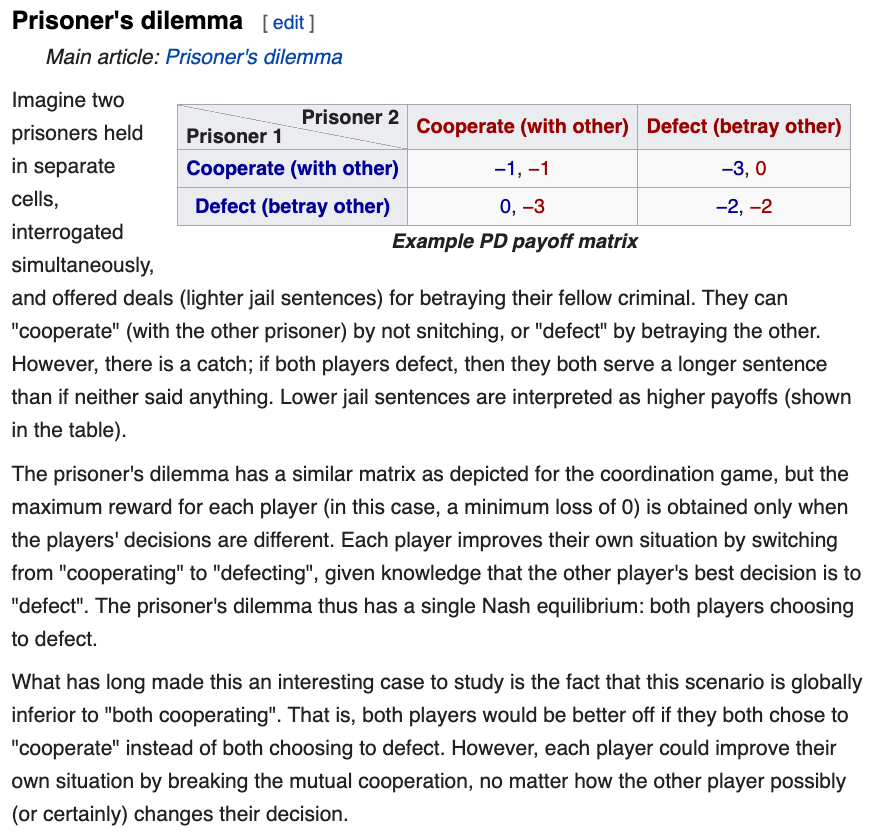
\includegraphics[width=8cm]{figures/PrisonersDilemma.png}
\end{frame}

\begin{frame}
  \frametitle{Driving Game}
  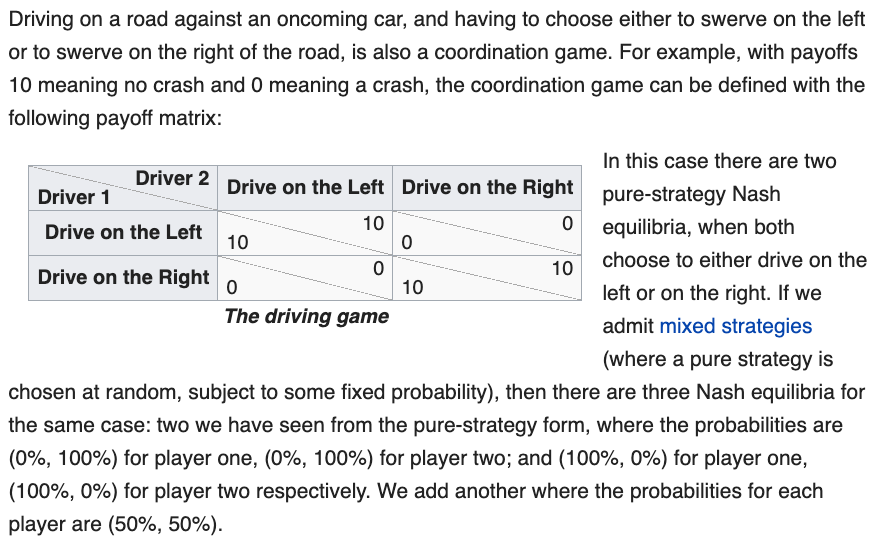
\includegraphics[width=8cm]{figures/DrivingGame.png}
\end{frame}

\begin{frame}
  \frametitle{Correlated Equilibrium}
  \begin{itemize}
  \item {\bf correlated equilibrium} proposed by Aumann [1974] much
    after {\bf Nash equilibrium} [1951] (earlier by Cournot [1838])
  \item A correlation device: a state that can be read by all players.
  \item Examples: counter, clock, stoplight.
  \item Strategy is a mapping from state of device to a distribution
    over actions.
  \end{itemize}
\end{frame}

\begin{frame}
  \frametitle{Game Of Chicken}
  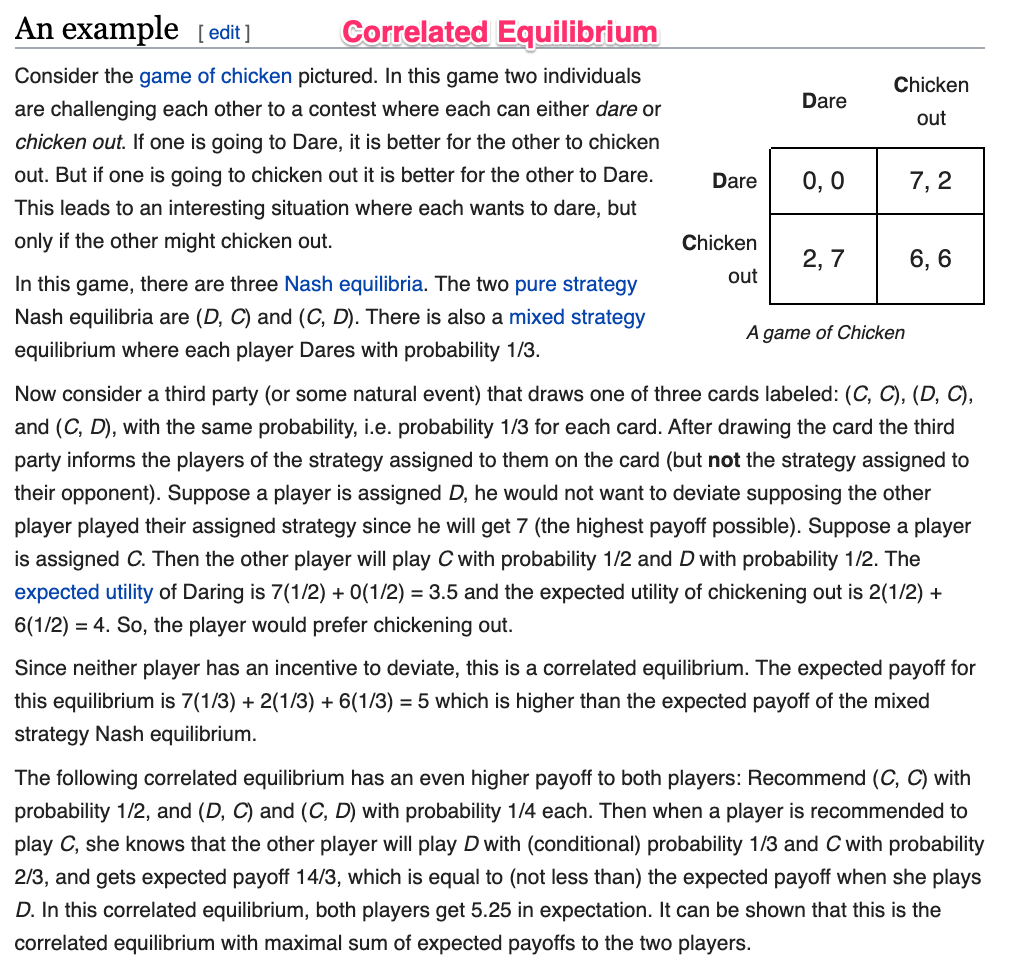
\includegraphics[width=8cm]{figures/CorrelatedEquilibrium.png}
\end{frame}

\section{Correlated equilibrium and Internal Regret}

\begin{frame}
  \frametitle{Finding the equilibrium mixed strategy}
  \begin{itemize}
  \item {\bf MiniMax} known matrix: Linear programming.
  \item {\bf MiniMax} Minimizing External Regret: Exponential weights or follow
    the perturbed leader.
  \item {\bf Nash equilibrium} known matrix - {\bf NP hard}
  \item {\bf Correlated Equilibrium} Minimizing Internal Regret.
  \end{itemize}
\end{frame}

\section{Calibration}
\begin{frame}
\frametitle{Calibration}
\begin{itemize}
\item Observe a binary sequence \R{$y_1,\ldots,y_{t-1}$} and make
  prediction \R{$q_t$} for the probability that \R{$y_t=1$}
\item Average outcomes: 
\R{
$$\rho_n^{\epsilon}(x) = 
\frac{\sum_{t=1}^n y_t {\bf 1}[q_t \in (x-\epsilon,x+\epsilon)]}
{\sum_{t=1}^n {\bf 1}[q_t \in (x-\epsilon,x+\epsilon)]}
$$}
\item $\epsilon$-calibrated predictions:
\R{
$$ \forall x \in [0,1];\;\; \limsup_{n \to \infty} \left|
  \rho_n^{\epsilon}(x) -x \right| \leq \epsilon
$$}
\item No deterministic algorithm can be calibrated for all sequences.
\end{itemize}
\end{frame}

\begin{frame}
\frametitle{Calibration through bounded internal regret}
\begin{itemize}
\item Consider only the predictions \R{$0,{1 \over N},{2 \over
      N},\ldots,{N \over N}$} for \R{$N>1$}
\item Use the square loss (Brier Loss) \R{$\sum_t (q_t - y_t)^2$}
\item Use a prediction algorithm that minimizes internal regret.
\item If the prediction is not $\epsilon$ calibrated, then the
  internal regret has to be large.
\end{itemize}
\end{frame}

\newcommand{\bp}{{\bf p}}

\section{Using an external regret algorithm to minimize internal regret}
\begin{frame}
\frametitle{From External to internal Regret}
\begin{itemize}
\item At time $t$ we need to produce a distribution \R{$\bp_t$} over
  \R{$N$} \B{actions}, so that the internal regret is small.
\item For each action pair \R{$i \neq j$} we define a 
{\em modified strategy} \R{$\bp_t^{i \to j}$} by setting the \R{$i$}th
coordinate in \R{$\bp_t$} to \R{$0$} and adding that mass to the
\R{$j$}th coordinate.
\item We use~ $\ouralg$ to combine the \R{$N(N-1)$} modified
  strategies. \R{$\sum_{i \neq j} \Delta_{(i,j),t} \bp_t^{i \to j}$}
\item But we need a distribution over \R{$N$} actions not \R{$N(N-1)$}
  modified strategies.
\item We solve the fixed point equation
\R{$$
\bp_t=
\sum_{i \neq j} \Delta_{(i,j),t} \bp_t^{i \to j} 
$$} 
\end{itemize}
\end{frame}

\end{document}


